%16/09 - Patricia Álvarez
\chapter{Máxima parsimonia - Cladística}
La cladística es un método de análisis de la sistemática filogenética que busca reconstruir las “genealogías” de los organismos y elaborar clasificaciones que las reflejen. Descansa sobre el axioma fundamental de que en la naturaleza, como resultado de la evolución, existe un orden que se manifiesta en las similitudes de los caracteres. Determina las relaciones evolutivas entre los organismos basándose en los caracteres relativamente derivados o apomórficos (novedades evolutivas). La reconstrucción filogenética consiste en identificar todos los grupos monofiléticos que existen en una muestra de taxones, que son aquellos definidos por sinapomorfías (caracteres derivados compartidos).

\section{Construir el árbol}
Desconocemos el aspecto del antecesor común más reciente de las especies y el modo en que están emparentadas, por lo que comenzamos a analizar sus relaciones buscando las diferentes formas en que pueden ser conectadas. Este ejemplo implica mayor similitud entre red (network) o árbol sin enraizar con ramificación dicotómica que conecta un grupo de taxones. No tiene raíz que conecte con un antecesor común; es como un mapa filogenético visto desde arriba, con el antecesor común oculto por sus descendientes. Es de ramificación dicotómica porque sólo tres ramas se juntan en cada unión o nodo; cada línea se divide siempre en dos ramas. Se pueden obtener otra red cambiando la posición de las especies. Existen tres posibles formas de unir 4 especies en una red de ramificación dicotómica. 

\begin{figure}[htbp]
\centering
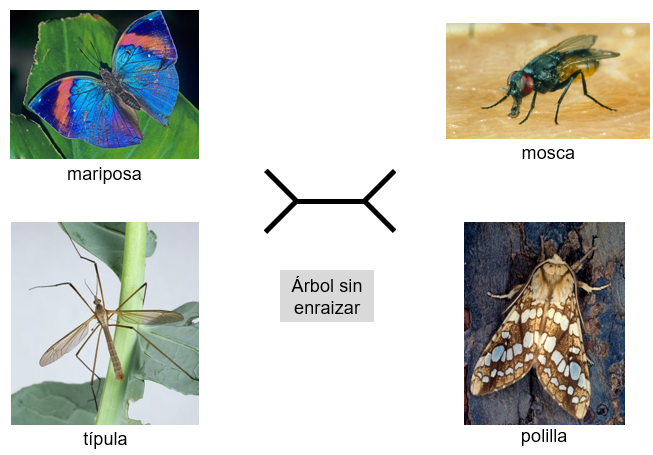
\includegraphics[width=0.5\linewidth]{figs/ejemplo-arbol-sin-enraizar.png}
\caption{Ejemplo de un árbol sin enraizar entre cuatro especies. Existen dos alternativas más árboles sin enraizar: mariposa-polilla con mosca-típula y mariposa-mosca con típula-polilla.}
\end{figure}

La selección de la explicación más sencilla de la distribución de los diferentes estados de caracteres se denomina \textbf{principio de parsimonia}. Así, se revisan los caracteres y se construye la matriz para ver cómo se sitúan los estados de los caracteres en las redes posibles. Aplicando el principio de parsimonia, se rechazan aquellos árboles que tengan más transformaciones en la red y se queda el más parsimonioso, es decir, el que necesita menos transformaciones evolutivas para explicar la distribución de los estados de los caracteres analizados. 

\begin{figure}[htbp]
\centering
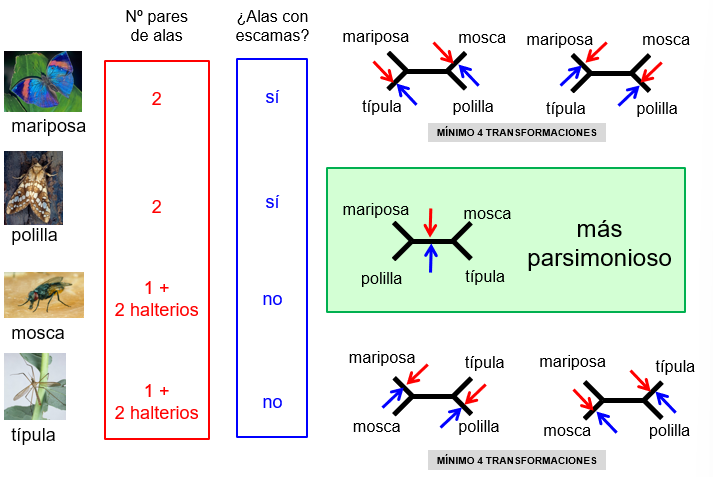
\includegraphics[width=0.5\linewidth]{figs/ejemplo-matriz-parsimonia.png}
\caption{Matriz de los estados de caracteres del ejemplo anterior. Tanto la mariposa como la polilla tienen dos pares de alas y las alas tienen escamas, mientras que la mosca y la típula tienen un par de alas y dos halterios y las alas no tienen escamas. A partir de ahí, se calculan las transformaciones necesarias para explicar la distribución del árbol y se elige el más parsimonioso, es decir, el que necesite un menor número de cambios.}
\end{figure}

Ante distintas hipótesis sobre las relaciones filogenéticas de los organismos dados, elegimos la más parsimoniosa, esto es, la que tenga una longitud menor (menor número de cambios), un mayor número de homologías y un menor número de homoplasias. Si hay varios árboles o hipótesis igualmente parsimoniosos, no podremos elegir entre ellos. La longitud de un árbol indica el número de transformaciones evolutivas necesarias para explicar los datos dada una topología de árbol concreta. Corresponde al número de cambios de estado que se producen en el árbol.

\section{Enraizar el árbol}
El siguiente paso es enraizar el árbol. La raíz nos permite determinar el lugar donde se encuentra el ancestro común. Para ello, se debe elegir la polaridad de los caracteres, es decir, conocer en qué orden se produjeron las transformaciones. Conocer qué estado del carácter es primitivo y cuál es derivado nos ayudará a elegir el cladograma con la distribución más sencilla de estados derivados (el más parsimonioso).

\begin{figure}[htbp]
\centering
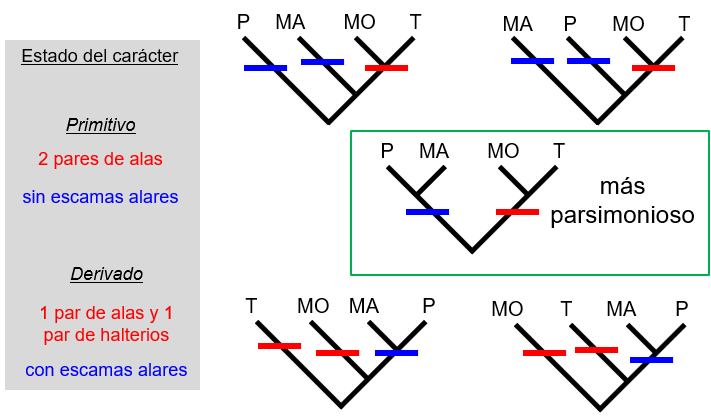
\includegraphics[width=0.5\linewidth]{figs/ejemplo-arbol-enraizado.png}
\caption{Opciones de árboles enraizados siguiendo el ejemplo anterior. Primero, sería importante conocer en qué orden se produjeron las transformaciones, si derivaron los halterios del segundo par de alas o si fue a la inversa. Supongamos que hay evidencias que sugieren que los halterios derivaron del segundo par de alas (que era el estado primitivo) y que la adquisición de escamas en las alas es otro estado de carácter derivado. En los posibles árboles, marcamos el lugar donde debe ocurrir la transformación de cada carácter de primitivo a derivado. El árbol más parsimonioso es aquel que necesita menos transformaciones para explicar la distribución de los estados derivados de los caracteres, y el que probablemente mejor registre las relaciones evolutivas de las cuatro especies de insectos.}
\end{figure}

La máxima parsimonia asume los siguientes principios: \begin{itemize}
\item \underline{Principio auxiliar de Hennig}: Ante caracteres similares y en ausencia de evidencia que indique evolución paralela o convergencia, siempre se asume que dichos caracteres son homólogos.
\item \underline{Regla de agrupación de Hennig}: Las sinapomorfías son evidencias de relaciones de ancestro común, mientras que las simplesiomorfías, las convergencias y los paralelismos no proporcionan evidencias sobre el ancestro común. 
\end{itemize}

Una auténtica homología debe circunscribir un grupo consistente con los especificados por otras homologías. Para comprobar esto, se realiza un \textbf{test de congruencia}. Así, se considera homología primaria cuando coincide, mientras que cuando se debe reinterpretar un carácter, se considera homología secundaria.

\begin{figure}[htbp]
\centering
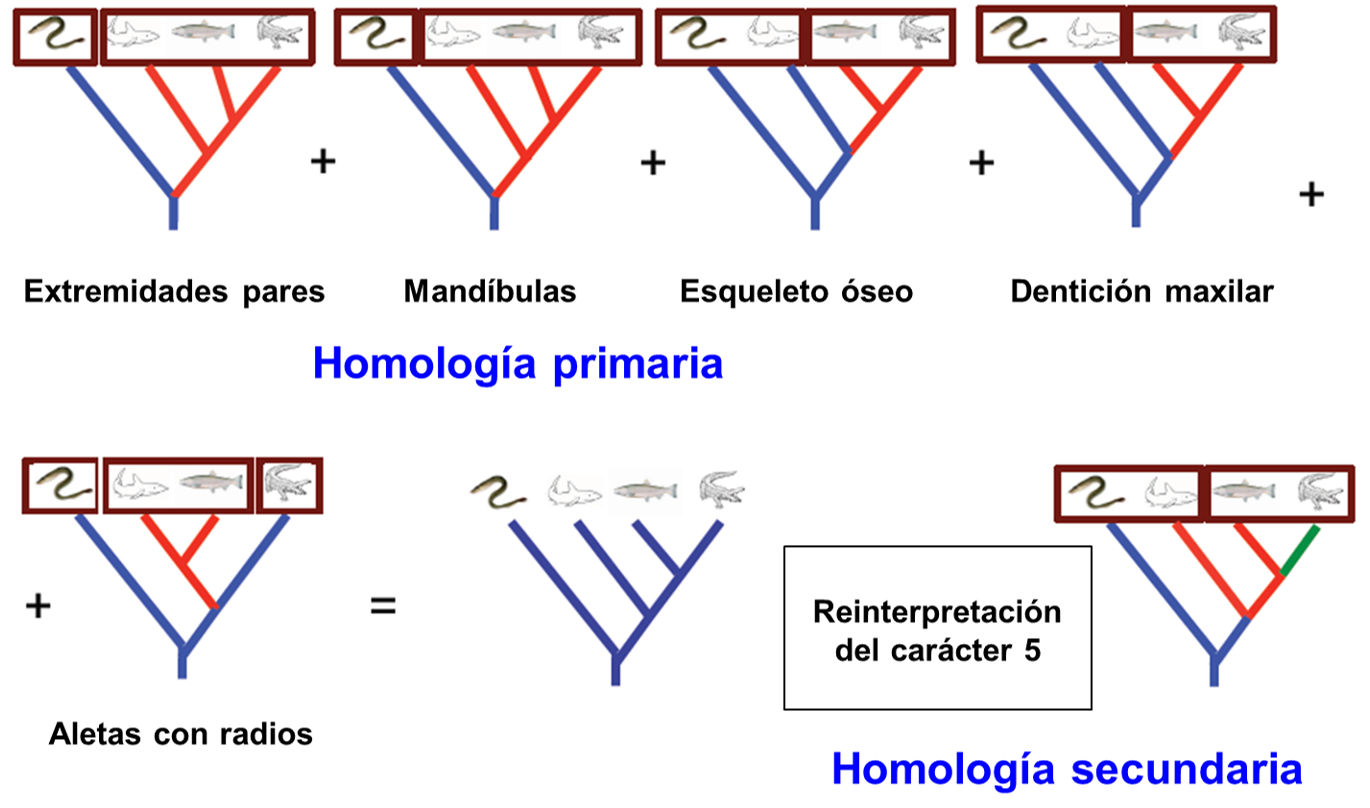
\includegraphics[width=0.5\linewidth]{figs/homologia-primaria-secundaria.png}
\caption{Árboles filogenéticos entre anguilas, tiburones, peces y cocodrilos basados en los caracteres de extremidades pares, mandíbulas, esqueleto óseo, dentición maxilar y aletas con radios. La mayoría de los árboles muestran una distribución similar de los taxones, mostrando así homología primaria. No obstante, el carácter aletas con radios es diferente, al relacionar dos taxones que en los demás caracteres no estaban relacionados. Ese carácter se debe reinterpretar, siendo así homología secundaria.}
\end{figure}

En el cladismo, se busca maximizar la congruencia entre caracteres, y así minimizar la incongruencia (homoplasia). En una aplicación computacional de la máxima parsimonia, se sigue un criterio de optimización (criterio para escoger entre diferentes cladogramas / relaciones filogenéticas), en el cual el cladograma preferido es aquél que tiene el menor número de transformaciones entre estados de carácter (pasos). Determinar los estados ancestrales implica poder identificar cambios de estado de carácter.

%lo dejamos aquí, lo siguiente es copia de las diapositivas
\section{Valoración de árboles}
Encontrar el cladograma más parsimonioso es la meta final de los análisis filogenéticos, aunque preguntas sobre su fiabilidad pueden permanecer. Para comparar objetivamente diferentes cladogramas y valorar el ajuste de los caracteres se han desarrollado medidas para cuantificar el alcance del problema de la homoplasia en los cladogramas obtenidos. Se comentan tres medidas: \begin{itemize}
\item Longitud del árbol: mide el número mínimo de transformaciones que se requieren en un determinado cladograma a partir de la matriz de caracteres (los árboles de longitud mínima para una matriz se llaman árboles de Wagner).
\item Índice de consistencia (CI): muestra la proporción de transformaciones que no se repiten (es decir, que no son homoplasias) en un cladograma.
\item Índice de retención (RI): estima el alcance de las sinapomorfías entre los estados de los caracteres en un cladograma determinado.
\item Índice de retención re-escalado (RCI): combina los dos anteriores, situando la homoplasia observada en una escala desde la mínima (0) a la máxima posible (1).
\end{itemize}
